\DiaryEntry{Group Theory, I}{2016-03-02}{algebra}


Groups are a generalization of structures such as the integers
\(\mathbb{Z}\) with addition or invertible \(2 \times 2\) matrices with
multiplication. However, groups can also represent ``actions'' or
operations such as permutations.

\subsection{Ressources}

\begin{itemize}

\item
  \href{https://en.wikibooks.org/wiki/Abstract_Algebra}{WikiBooks}
\item
  \href{http://groupprops.subwiki.org/wiki/Main_Page}{Group Wiki}
\item
  \href{http://abstract.ups.edu/download.html}{Abstract Algebra} with
  \href{https://github.com/twjudson/aata}{source}
\end{itemize}

\subsection{Group Definition}

Consider a function \(G \times G \rightarrow G\) that assigns each pair
\((a,b) \in G \times G\) a unique element \(a \star b \in G\). The
function is called binary operation or law of composition; the result is
called the composition of \(a\) and \(b\).

A group \((G, \star)\) is a set \(G\) with a law of composition that
satisifies the following axioms:

\begin{itemize}
\item
  The function is associative:
  \((a \star b) \star c = a \star (b \star c)\)
\item
  There exists an identity element \(e\) so that
  \(e \star a = a \star e = a\) for any \(a \in G\).
\item
  There exists an inverse element \(a^{-1}\) so that
  \(a a^{-1} = a^{-1} a = e\) for any \(a \in G\).
\end{itemize}

A group need not be commutative (i.e. \(a \star b = b \star a\)); if it
is, the group is called abelian.

\subsubsection{Example: Integers mod n
Addition}\label{example-integers-mod-n-addition}

The integers modulo n form a group under addition modulo n. Consider
\(\mathbb{Z}_5\); i.e.~the integers modulo \(5\). The addition table is
given as

\begin{figure}
\centering
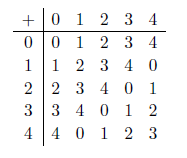
\includegraphics{images/groups_01_1.png}
\caption{Page1}
\end{figure}

The effect of the identitiy element \(0\) can be seen in the first row /
column. Furthermore, \(0\) appears exactely once in every row / column;
therefore there exists an inverse element.

\subsubsection{Example: Integers mod n
Multiplication}\label{example-integers-mod-n-multiplication}

If we consider modulo n multiplication instead, things become different:
The element \(1\) acts as identitiy element \(a \star 1 = a\), but there
is no inverse element for the element \(0\): \(a \star 0 = 0\) for all
\(a\). The way out of this is to remove the element \(0\); i.e.~we
consider \(\mathbb{Z}_n - \{0\}\).

This remedy does not create a group in all cases \(n\) as the following
example shows: The table below shows the multiplication tables for
\(\mathbb{Z}_4 - \{0\}\) and \(\mathbb{Z}_5 - \{0\}\).

\begin{figure}
\centering
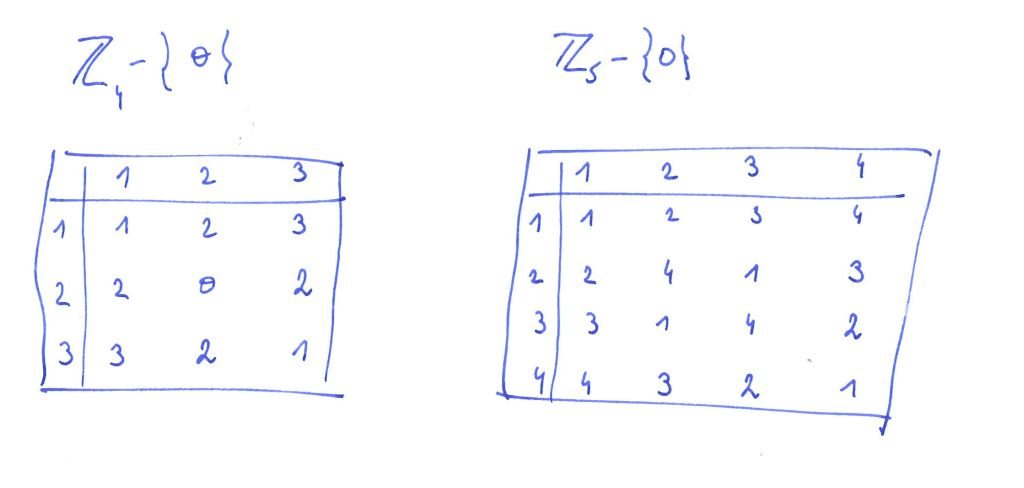
\includegraphics{images/groups_01_2.jpg}
\caption{Page1}
\end{figure}

\(\mathbb{Z}_4 - \{0\}\) has no identitiy element for \(2\); no matter
what \(2\) is multiplied with, the result is never \(1\) (the identity
element). Furthermore, \(0\) is per definition \textbf{not} an element
of \(\mathbb{Z}_4 - \{0\}\). Therefore, \(\mathbb{Z}_4 - \{0\}\) is
\textbf{not} a group. For \(\mathbb{Z}_5 - \{0\}\), every element has an
inverse; therefore this set forms a group (under multiplication module
\(5\)).

There is a proposition, that every nonzero \(k\) has an inverse in
\(\mathbb{Z}_n - \{0\}\), if \(k\) is relatively prime to \(n\). If we
collect all elements \(k \in \mathbb{Z}_n - \{0\}\) which have
\(\gcd(k,n)=1\), we obtain a group, the \textbf{group of units} \(U(n)\)
of \(\mathbb{Z}_n\). Euler's totient function \(\phi(n)\) counts the
integers up to a given number n that are relatively prime to n.
Therefore, the group of units order is \(|U(n)| = \phi(n)\).

As an example consider \(n=8\): The following elements of
\(\mathbb{Z}_8 - \{0\}\) are relatively prime to 8: 1,3,5,7. These
elements form the group of unity \(U(8)\) which multiplication table is
as follows:

\[
\begin{array}{c|cccc}
\star & 1 & 3 & 5 & 7 \\ \hline
1     & 1 & 3 & 5 & 7 \\
3     & 3 & 1 & 7 & 5 \\
5     & 5 & 7 & 1 & 3 \\
7     & 7 & 5 & 3 & 1
\end{array}
\]

Finally, if \(n\) is prime, then all \(k\) are relatively prime to \(n\)
and the set \(\mathbb{Z}_n - \{0\}\) forms a group under multiplication
modulo n. This is the reason why \(\mathbb{Z}_5 - \{0\}\) is a group.

\subsection{Subgroups}\label{subgroups}

A subgroup \(H\) of a group \(H\) is a subset \(H\) of \(G\) such that
when the group operation of \(G\) is restricted to \(H\), \(H\) is a
group in its own right. Every group \(G\) with at least 2 elements has
always two subgroups: the subgroup containing the identity element only
(trivial subgroup) and the group \(G\) itself. Everything in between is
a proper subgroup.

\subsection{Cyclic (Sub)Groups}\label{cyclic-subgroups}

If \(G\) is a group and \(a\) any element of the group. Then the set

\[
\langle a \rangle = \{a^k: k \in \mathbb{Z}\}
\]

is a subgroup of \(G\) and \(\langle a \rangle\) is the smallest
subgroup of \(G\) that contains \(a\).

Note that \(a^k\) denotes repeated (k times) application of the
\(\star\) operation on \(a\). I.e.
\(a^2 = a \star a, a^3 = a \star a \star a \cdots\). If using \(+\) as a
group operation, then \(\langle a \rangle = \{ka: k \in \mathbb{Z}\}\)
will be more intuitive.

Proof: \(k=0 \rightarrow a^0 = e\) creates the identity element which is
in \(\langle a \rangle\). If \(g = a^m\) and \(h = a^n\), then
\(g \star h = a^{m+n} \in \langle a \rangle\) (the subgroup is closed)
and finally, \(a^n \star a^{-n} = e\), i.e.~for every
\(a \in \langle a \rangle\), there exists an inverse element.

There are two options for the relation between \(\langle a \rangle\) and
G:

\begin{itemize}
\item
  \(\langle a \rangle\) is a subgroup of G; in this case
  \(\langle a \rangle\) is called a \textbf{cyclic subgroup} of G.
\item
  \(\langle a \rangle\) = G; i.e.~the complete group G can be created
  via the cyclic operation. In this case, G is called a \textbf{cyclic
  group} and and a is the \textbf{generator} of G.
\end{itemize}

The sequence \(e, a, a^2, a^3, \cdots\) may eventually end in the
identity element \(e\). In this case we speak of finite cyclic
(sub)groups. The order of \(\langle a \rangle\) is the smallest positive
integer n such that \(a^n = e\).

As an example, consider the group \(\mathbb{Z}_5\) (addition module-5).
The element \(1\) is a generator for the group:
\(0 \times 1 = 0, 1 \times 1 = 1, 2 \times 1 = 2, 3 \times 1 = 3, 4 \times 1 = 4, 5 \times 1 = 0\).
Therefore, \(\mathbb{Z}_5\) is a cyclic group with order 5. In the same
spirit, the element \(2\) is also a generator for the group:
\(0 \times 2 = =0, 1 \times 2 = 2, 2 \times 2 = 4, 3 \times 2 = 1, 4 \times 2 = 3, 5 \times 2 = 0\).

The generator \(2\) of the group \(\mathbb{Z}_6\) creates a cyclic
subgroup \(\langle 2 \rangle = \{0, 2, 4\}\) which does not equal the
group. So \(\langle 2 \rangle\) is a cyclic subgroup of order 3.
